%%%%%%%%%%%%%%%%%%%%%%%%%%%%%%%%%%%%%%%%%
% Beamer Presentation
% LaTeX Template
% Version 1.0 (10/11/12)
%
% This template has been downloaded from:
% http://www.LaTeXTemplates.com
%
% License:
% CC BY-NC-SA 3.0 (http://creativecommons.org/licenses/by-nc-sa/3.0/)
%
%%%%%%%%%%%%%%%%%%%%%%%%%%%%%%%%%%%%%%%%%

%----------------------------------------------------------------------------------------
%	PACKAGES AND THEMES
%----------------------------------------------------------------------------------------

\documentclass{beamer}

\mode<presentation> {

% The Beamer class comes with a number of default slide themes
% which change the colors and layouts of slides. Below this is a list
% of all the themes, uncomment each in turn to see what they look like.

%\usetheme{default}
%\usetheme{AnnArbor}
%\usetheme{Antibes}
%\usetheme{Bergen}
%\usetheme{Berkeley}
%\usetheme{Berlin}
%\usetheme{Boadilla}
%\usetheme{CambridgeUS}
%\usetheme{Copenhagen}
%\usetheme{Darmstadt}
%\usetheme{Dresden}
%\usetheme{Frankfurt}
%\usetheme{Goettingen}
%\usetheme{Hannover}
%\usetheme{Ilmenau}
%\usetheme{JuanLesPins}
%\usetheme{Luebeck}
\usetheme{Madrid}
%\usetheme{Malmoe}
%\usetheme{Marburg}
%\usetheme{Montpellier}
%\usetheme{PaloAlto}
%\usetheme{Pittsburgh}
%\usetheme{Rochester}
%\usetheme{Singapore}
%\usetheme{Szeged}
%\usetheme{Warsaw}
\colorlet{beamer@blendedblue}{red!60!black}


% As well as themes, the Beamer class has a number of color themes
% for any slide theme. Uncomment each of these in turn to see how it
% changes the colors of your current slide theme.

%\usecolortheme{albatross}
%\usecolortheme{beaver}
%\usecolortheme{beetle}
%\usecolortheme{crane}
%\usecolortheme{dolphin}
%\usecolortheme{dove}
%\usecolortheme{fly}
%\usecolortheme{lily}
%\usecolortheme{orchid}
%\usecolortheme{rose}
%\usecolortheme{seagull}
%\usecolortheme{seahorse}
%\usecolortheme{whale}
%\usecolortheme{wolverine}

%\setbeamertemplate{footline} % To remove the footer line in all slides uncomment this line
%\setbeamertemplate{footline}[page number] % To replace the footer line in all slides with a simple slide count uncomment this line

%\setbeamertemplate{navigation symbols}{} % To remove the navigation symbols from the bottom of all slides uncomment this line
}

\usepackage{graphicx} % Allows including images
\usepackage{booktabs} % Allows the use of \toprule, \midrule and \bottomrule in tables
\usepackage{multirow}
\usepackage{multicol}
\usepackage{adjustbox}
\usepackage{array}
\usepackage{tikz}
\usepackage{soul}
\usetikzlibrary{shapes.geometric, arrows, positioning, fit}
\usepackage[latin1]{inputenc}
\newcommand{\xmark}{\textcolor{red}{\text{\sffamily X}}}
\newcommand{\cmark}{\textcolor{green}{\checkmark}}
\newcommand{\tr}{\text{tr}}
\newcommand{\E}{\textbf{E}}
\newcommand{\diag}{\text{diag}}
\newcommand{\argmax}{\text{argmax}}
\newcommand{\argmin}{\text{argmin}}
\newcommand{\Cov}{\text{Cov}}
\newcommand{\Var}{\text{Var}}
\newcommand{\Vol}{\text{Vol}}
\newcommand{\bx}{\boldsymbol{x}}
\newcommand{\by}{\boldsymbol{y}}
\newcommand{\bX}{\boldsymbol{X}}
\newcommand{\bY}{\boldsymbol{Y}}
\sethlcolor{gray}
\makeatletter
\newcommand\SoulColor{%
  \let\set@color\beamerorig@set@color
  \let\reset@color\beamerorig@reset@color}
\makeatother
\definecolor{color1}{RGB}{128,13,13}
\definecolor{color2}{RGB}{70,128,13}
\definecolor{color3}{RGB}{13,128,128}
\definecolor{color4}{RGB}{70,13,128}


\newcommand{\faceA}{
\includegraphics[scale = 0.15]{face_photos/Amelia_Vega_0002.png}}
\newcommand{\faceB}{
\includegraphics[scale = 0.15]{face_photos/Jean-Pierre_Raffarin_0004.png}}
\newcommand{\faceC}{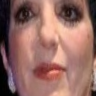
\includegraphics[scale = 0.15]{face_photos/Liza_Minnelli_0003.png}}
\newcommand{\faceD}{
\includegraphics[scale = 0.15]{face_photos/Patricia_Clarkson_0001.png}}

%tikz stufff


%----------------------------------------------------------------------------------------
%	TITLE PAGE
%----------------------------------------------------------------------------------------


%Extrapolating prediction error for 'extreme' multi-class classification

%with Rakesh Achanta and Yuval Benjamini

%'Extreme' classification refers to the classification with extremely
%large (on the order of millions) of labels, such as in photo or
%website annotation.  A natural question in these settings is whether
%the data is sufficiently rich to support high-accuracy classification
%with such a large label space.  Therefore, in this work, we address
%the question of predicting how well a classifier will scale with an
%increased number of classes, based on its performance in a smaller but
%representative classification problem. Under the assumption that the
%classes are sampled exchangeably, and under the assumption that the
%classifier is based on marginal probabilities (e.g. QDA or Naive
%Bayes), we derive a method for performance extrapolation based on
%unbiased estimation. We investigate the robustness of our methods to
%non-marginal classifiers in simulations and one optical character
%recognition example.


% Image sources
% http://sociable.co/social-media/how-to-disable-facebook-facial-recognition/
% https://alexanderskv.wordpress.com/2012/06/04/facial-recognition/
% https://medium.com/@ageitgey/machine-learning-is-fun-part-4-modern-face-recognition-with-deep-learning-c3cffc121d78#.fzgvan3ii

\title[Defense]{Supervised Evaluation of Representations}

\author{Charles Zheng} % Your name
\institute[Stanford] % Your institution as it will appear on the bottom of every slide, may be shorthand to save space
{Stanford University}
\date{\today} % Date, can be changed to a custom date

\begin{document}

\begin{frame}
\titlepage % Print the title page as the first slide
%(Joint work with Rakesh Achanta and Yuval Benjamini.)
\end{frame}

\section{Randomized Classification}

\begin{frame}
\sectionpage
\end{frame}


\begin{frame}
\frametitle{Facial recognition problem}
Let's say I have a database of users, $i = 1,\hdots,k$, with photos $\vec{z}_j$ that are labelled.
%Kay (2008) image identification task in functional MRI.
\begin{center}
%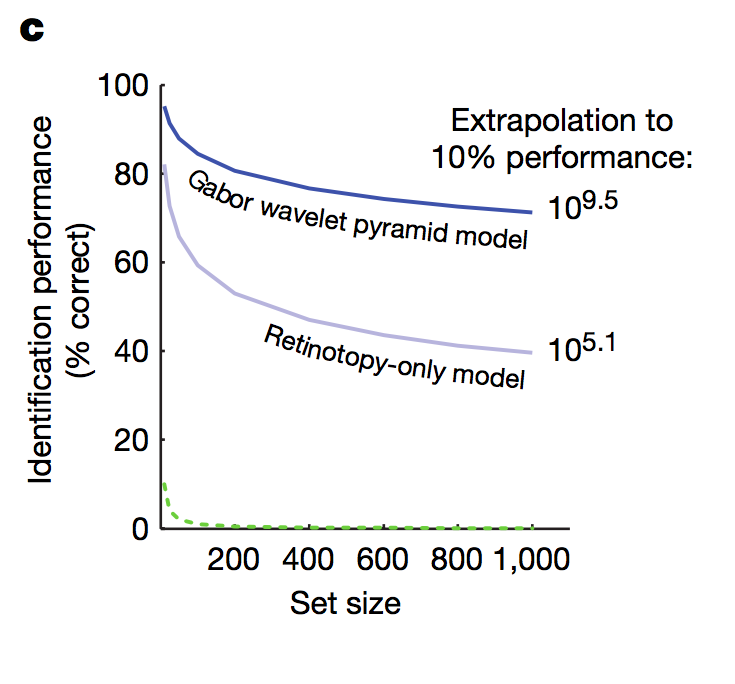
\includegraphics[scale = 0.2, clip=true, trim = 0 0in 0 0]{kay_extrapolation.png}
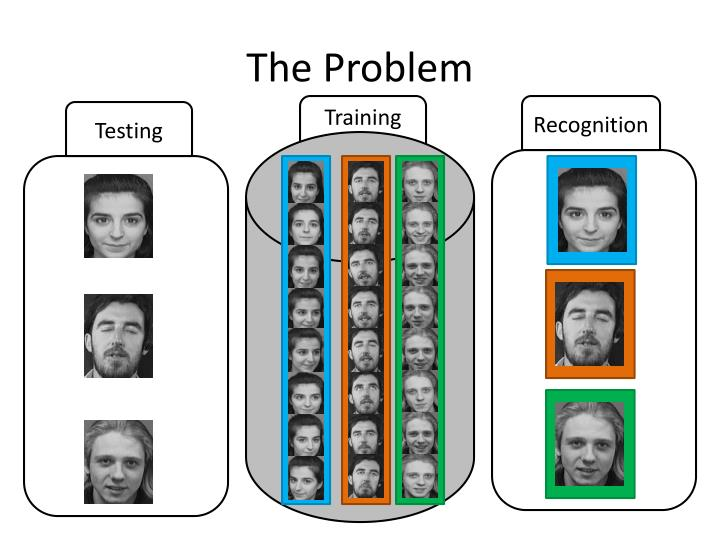
\includegraphics[scale = 0.2]{face_rec_the-problem-n.jpg}\pause
\hspace{0.2in}
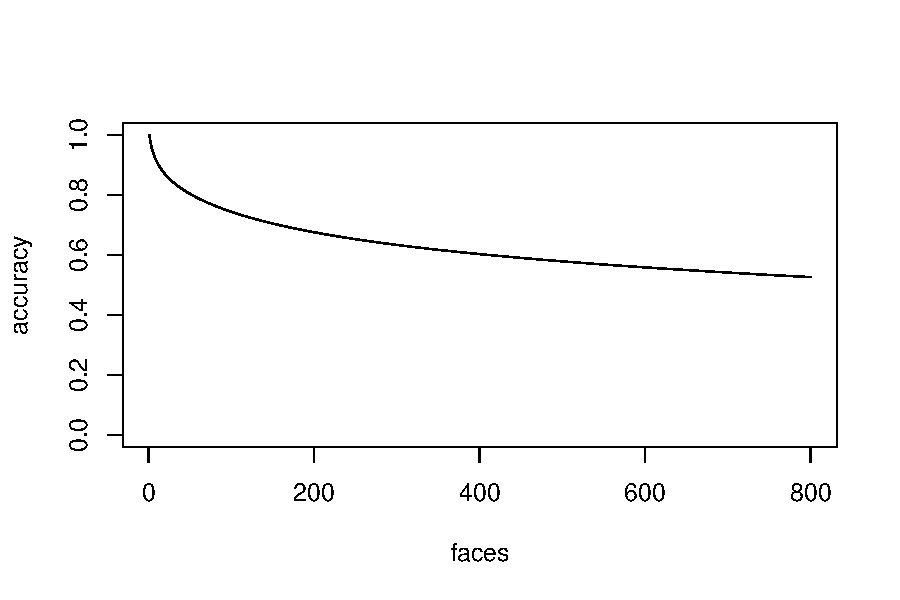
\includegraphics[scale = 0.3]{../facerec/acc_plot1.pdf}\pause
\end{center}

How does the accuracy scale with the number of classes (faces)?
\end{frame}




\begin{frame}
\frametitle{Setup}

\begin{center}
\begin{tabular}{c|c}
1. Population of categories $\pi(y)$ & 
2. Subsample $k$ labels, $y_1,\hdots, y_k$\\
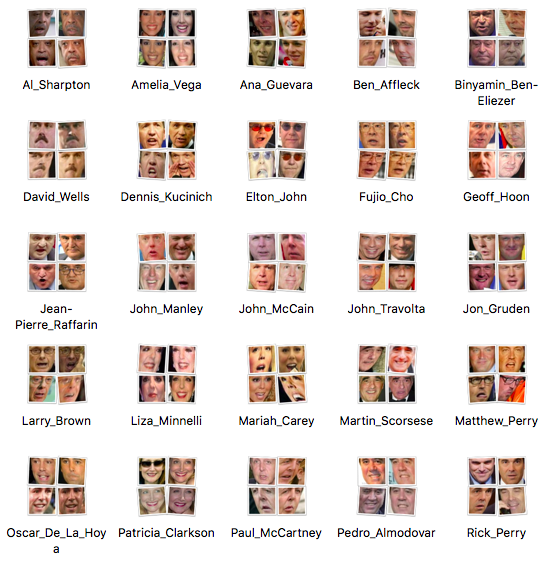
\includegraphics[scale = 0.2]{photo_folders.png} &
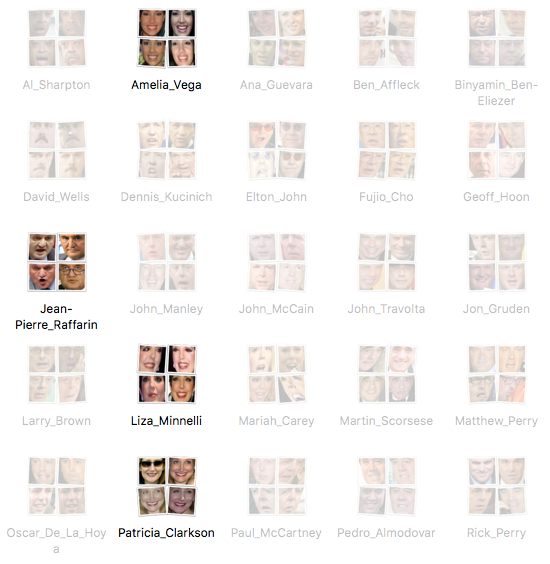
\includegraphics[scale = 0.2]{photo_folders2.png}
\end{tabular}
\end{center}

\end{frame}



\begin{frame}
\frametitle{Setup}

\vspace{0.1in}
3. Collect training and test data $x_j^{(i)}$ (faces) for labels (people) $\{y_1,\hdots, y_k\}$.

\begin{center}
\begin{tabular}{|c|ccc|c|}
\hline
Label & & Training & & Test\\ \hline
$y_1$=Amelia & 
  $x_1^{(1)} = $
\includegraphics[scale = 0.2]{face_photos/Amelia_Vega_0001.png} &  
  $x_1^{(2)} = $
\includegraphics[scale = 0.2]{face_photos/Amelia_Vega_0002.png} &  
  $x_1^{(3)} = $
\includegraphics[scale = 0.2]{face_photos/Amelia_Vega_0003.png} &  
  $x_1^{*} = $
\includegraphics[scale = 0.2]{face_photos/Amelia_Vega_0004.png} \\ \hline
$y_2$=Jean-Pierre & 
  $x_2^{(1)} = $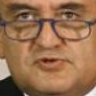
\includegraphics[scale = 0.2]{face_photos/Jean-Pierre_Raffarin_0001.png} &  
  $x_2^{(2)} = $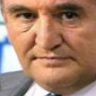
\includegraphics[scale = 0.2]{face_photos/Jean-Pierre_Raffarin_0002.png} &  
  $x_2^{(3)} = $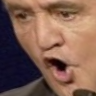
\includegraphics[scale = 0.2]{face_photos/Jean-Pierre_Raffarin_0003.png} &  
  $x_2^{*} = $
\includegraphics[scale = 0.2]{face_photos/Jean-Pierre_Raffarin_0004.png} \\ \hline
$y_3$=Liza & 
  $x_3^{(1)} = $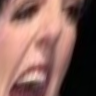
\includegraphics[scale = 0.2]{face_photos/Liza_Minnelli_0001.png} &  
  $x_3^{(2)} = $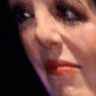
\includegraphics[scale = 0.2]{face_photos/Liza_Minnelli_0002.png} &  
  $x_3^{(3)} = $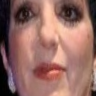
\includegraphics[scale = 0.2]{face_photos/Liza_Minnelli_0003.png} &  
  $x_3^{*} = $
\includegraphics[scale = 0.2]{face_photos/Liza_Minnelli_0004.png} \\ \hline
$y_4$=Patricia & 
  $x_4^{(1)} = $
\includegraphics[scale = 0.2]{face_photos/Patricia_Clarkson_0001.png} &  
  $x_4^{(2)} = $
\includegraphics[scale = 0.2]{face_photos/Patricia_Clarkson_0002.png} &  
  $x_4^{(3)} = $
\includegraphics[scale = 0.2]{face_photos/Patricia_Clarkson_0003.png} &  
  $x_4^{*} = $
\includegraphics[scale = 0.2]{face_photos/Patricia_Clarkson_0004.png} \\ \hline
\end{tabular}
\end{center}


\vspace{0.1in}
4. Train a classifier and compute test error. \pause

\vspace{0.1in}
\textbf{Can we analyze how error depends on }$k$?
\end{frame}


\begin{frame}
\frametitle{Key assumption: marginal classifier}
\begin{itemize}
\item The classifier is \emph{marginal} if it learns a model \emph{independently} for each class.\pause
\item Examples: LDA/QDA 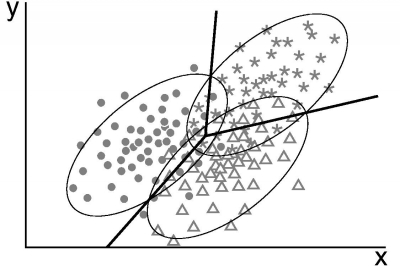
\includegraphics[scale = 0.2]{discriminant.jpg}, \pause
na\"{i}ve Bayes 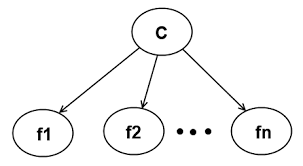
\includegraphics[scale = 0.2]{naive_bayes.png} \pause
\item Non-marginal classifiers: Multinomial logistic, multilayer neural networks, k-nearest neighbors
\end{itemize}
\end{frame}

\begin{frame}
\frametitle{Definitions}

$\hat{F}_{y^{(i)}}$ is the empirical distribution obtained from the training data for label $y^{(i)}$.

\begin{center}
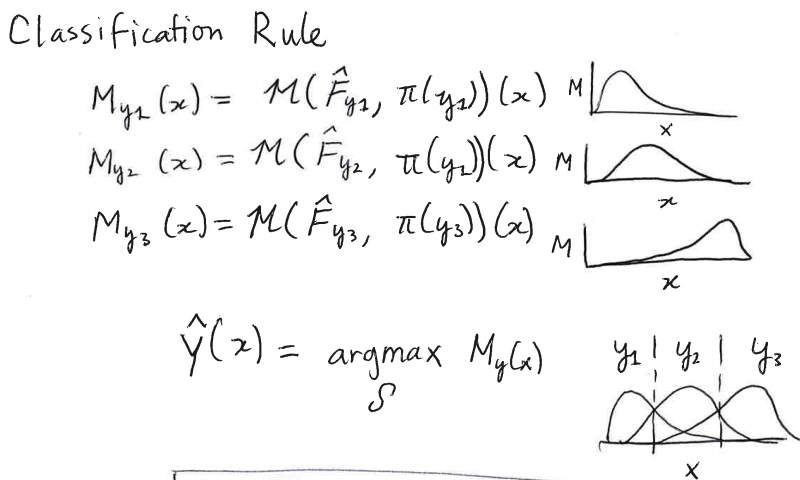
\includegraphics[scale = 0.2]{../info_theory_paper/extrapolation_figures/classification_rule.png}
\end{center}
\end{frame}

\begin{frame}

\begin{center}
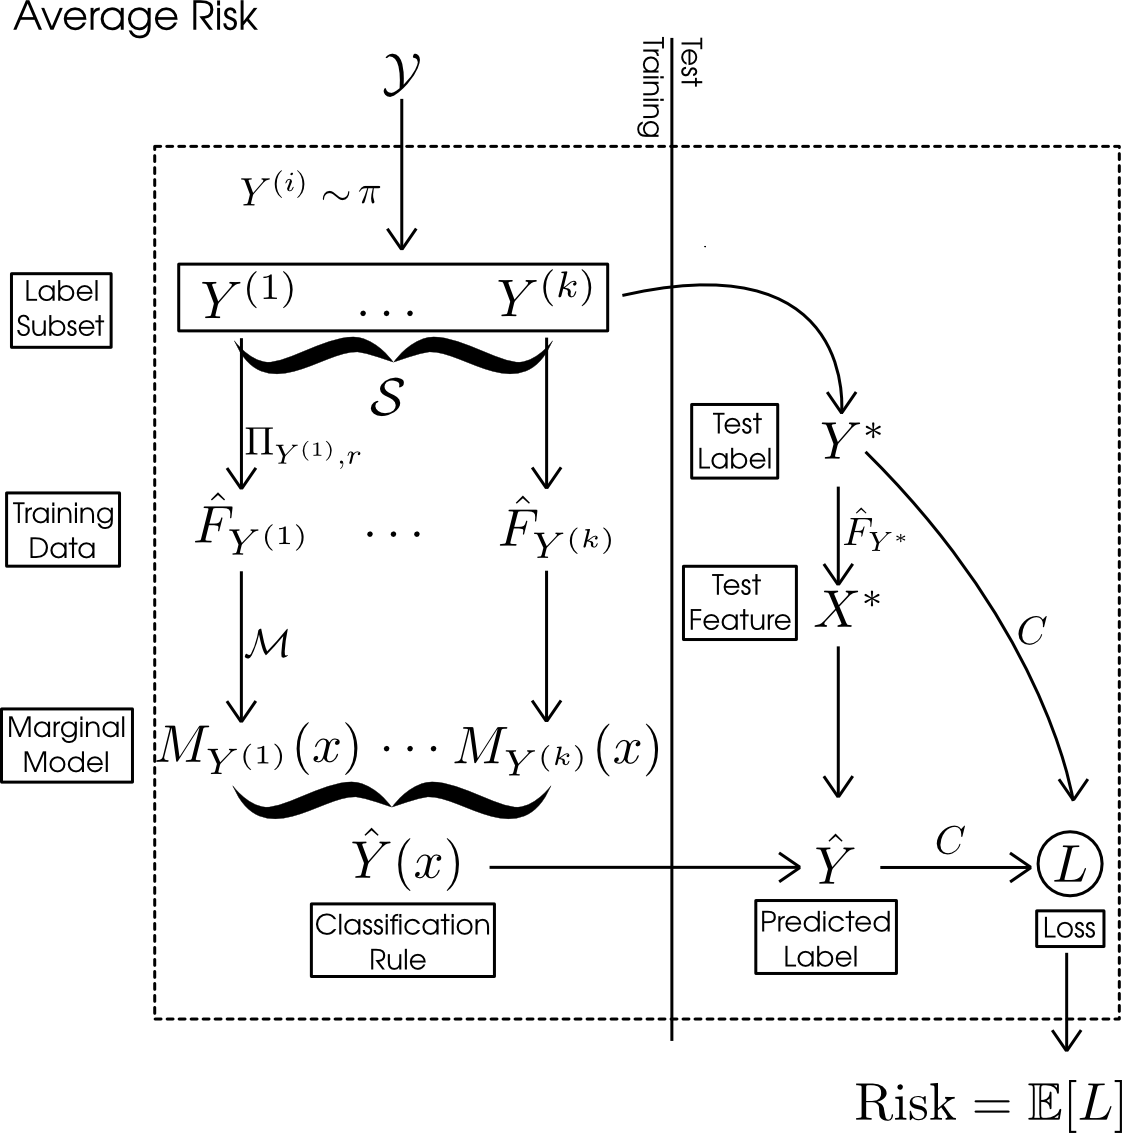
\includegraphics[scale = 0.2]{../info_theory_paper/extrapolation_figures/average_risk.png}
\end{center}
\end{frame}


\begin{frame}
\frametitle{Theoretical Result}

\textbf{Theorem. (Z.}, Achanta, Benjamini.)
Suppose $\pi$, $\{F_y\}_{y \in \mathcal{Y}}$ and marginal classifier
$\mathcal{F}$ satisfy \emph{(some regularity condition)}.  Then, 
there exists some function $\bar{D}(u)$ on $[0,1] \to [0,1]$ such that
the $k$-class average risk is given by
\[
\text{AvRisk}_k = (k-1) \int \bar{D}(u) u^{k-2} du.
\]
\pause

\vspace{1in}
What is this $\bar{D}(u)$ function? We will explain in the following toy example...
\end{frame}

\begin{frame}
\frametitle{Toy example}
$Y_1,\hdots, Y_k \stackrel{iid}{\sim} N(0, 1);$\pause

$X|Y \sim N(\rho Y, 1-\rho^2)$ i.e. $(Y, X) \sim N(0, \begin{pmatrix}1 & \rho\\\rho & 1\end{pmatrix}).$

\begin{center}
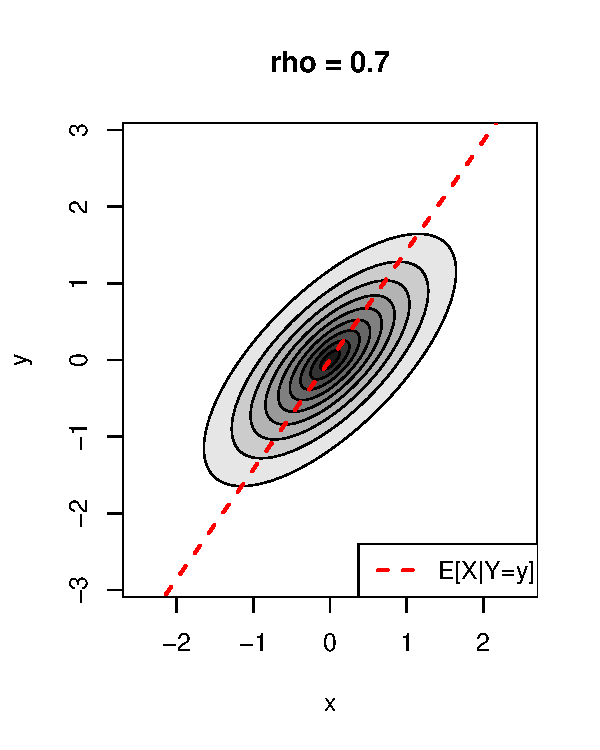
\includegraphics[scale = 0.5, clip = true, trim = 0 0 0 0.5in]{../extrapolation/illus_rho_0_7.pdf}
\end{center}

\end{frame}





\begin{frame}
\frametitle{Toy example}

\begin{center}
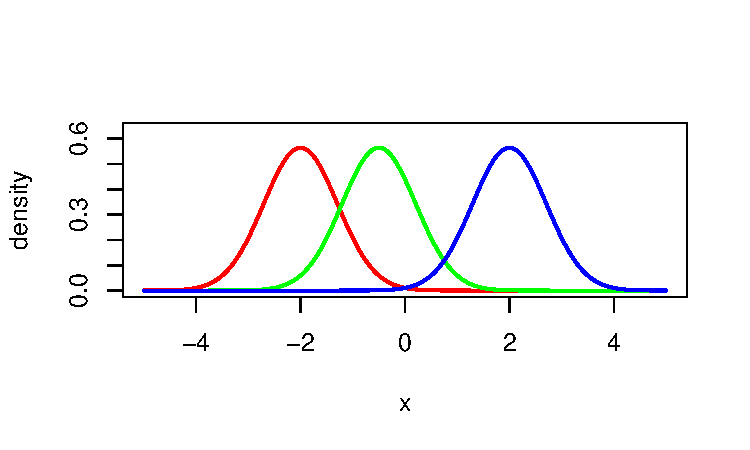
\includegraphics[scale = 0.5, clip = true, trim = 0 0.8in 0 0.8in]{../extrapolation/illus_example1a.pdf}
\end{center}

\begin{itemize}
\item Suppose $k=3$, and we draw $Y_1, Y_2, Y_3$.
\item The \emph{Bayes rule} is the optimal classifier and depends on knowing the true densities:
\[
\hat{y}(x) = \text{argmax}_{y_i} p(x|y_i)
\]
\item The \emph{Bayes Risk}, which is the misclassification rate of the optimal classifier.
\end{itemize}

\end{frame}

\begin{frame}
\frametitle{Toy example}

\begin{center}
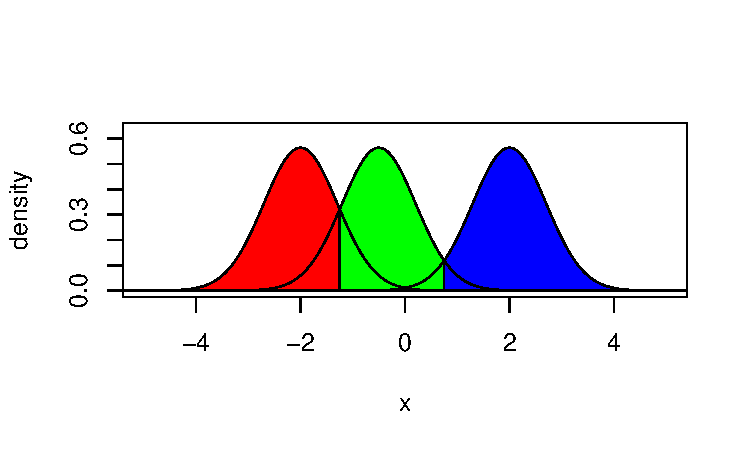
\includegraphics[scale = 0.5, clip = true, trim = 0 0 0 0.5in]{../extrapolation/illus_example1b.pdf}
\end{center}

\begin{itemize}
\item The \emph{Bayes Risk} is the expected test error of the Bayes rule,
\[
\frac{1}{k} \sum_{i=1}^k \Pr[\hat{y}(x) \neq Y| Y = y_i]
\]
\end{itemize}
% = 1 - \frac{1}{k}\int \max_{i=1}^k p(x|y_i) dx.

\end{frame}

\begin{frame}
\frametitle{Toy example}
\begin{columns}
\begin{column}{0.5\textwidth}
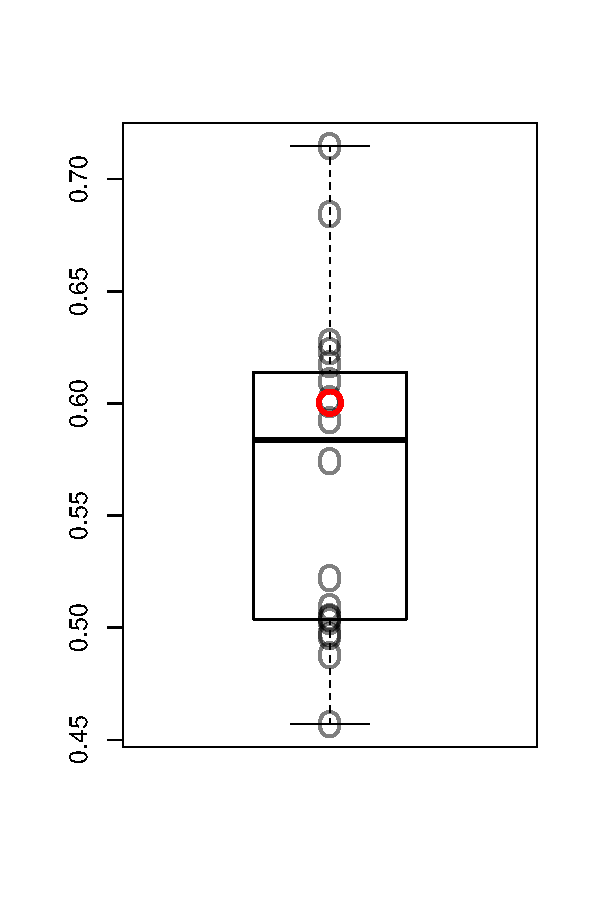
\includegraphics[scale = 0.5]{../extrapolation/autoplots/box4_1.pdf}
\end{column}
\begin{column}{0.5\textwidth}
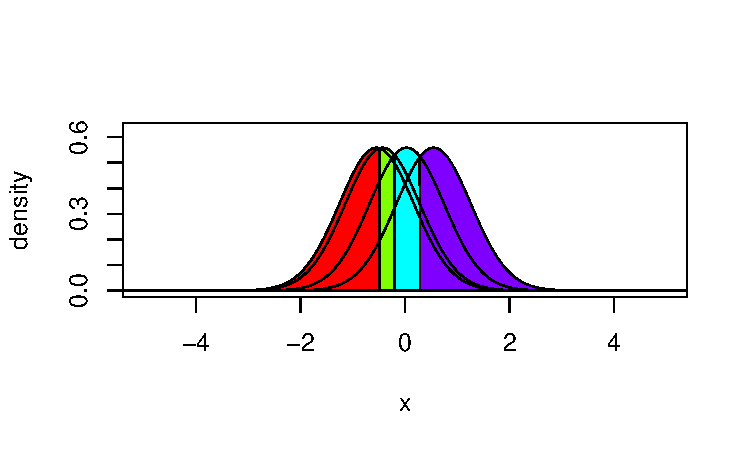
\includegraphics[scale = 0.5]{../extrapolation/autoplots/dens4_1.pdf}
\end{column}
\end{columns}
\end{frame}

\begin{frame}
\frametitle{Toy example}
\begin{columns}
\begin{column}{0.5\textwidth}
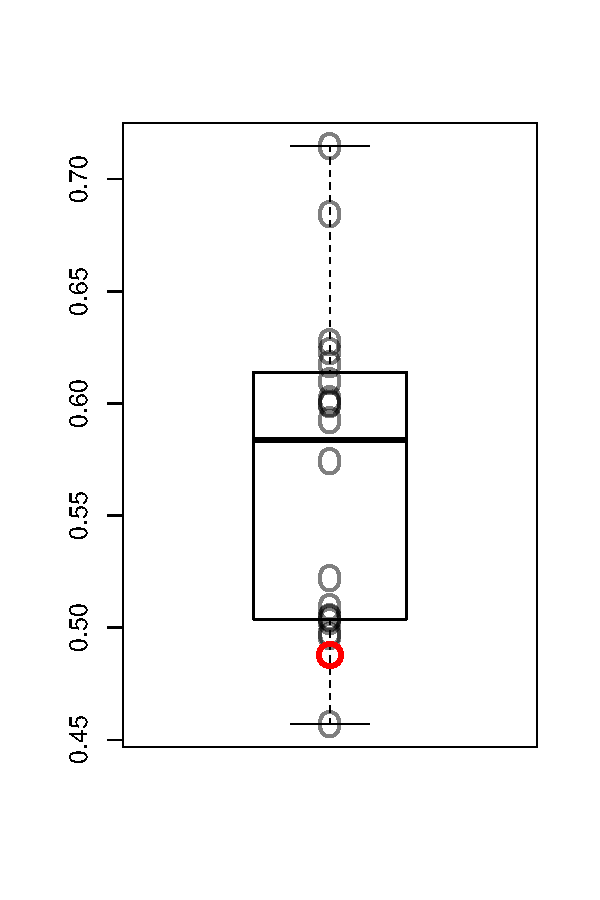
\includegraphics[scale = 0.5]{../extrapolation/autoplots/box4_2.pdf}
\end{column}
\begin{column}{0.5\textwidth}
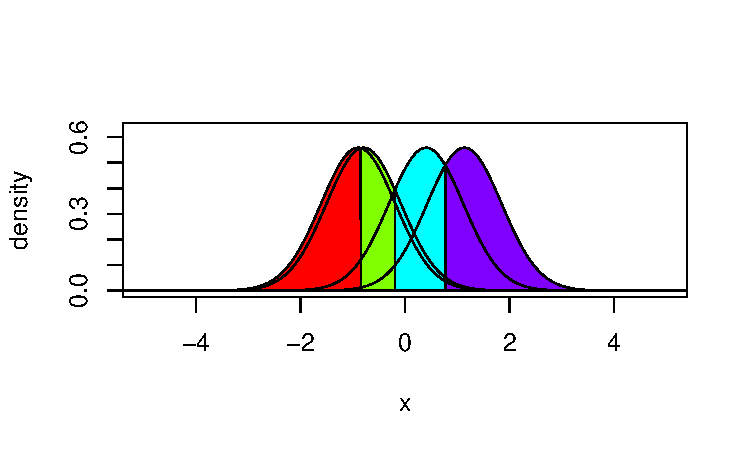
\includegraphics[scale = 0.5]{../extrapolation/autoplots/dens4_2.pdf}
\end{column}
\end{columns}
\end{frame}

\begin{frame}
\frametitle{Toy example}
\begin{columns}
\begin{column}{0.5\textwidth}
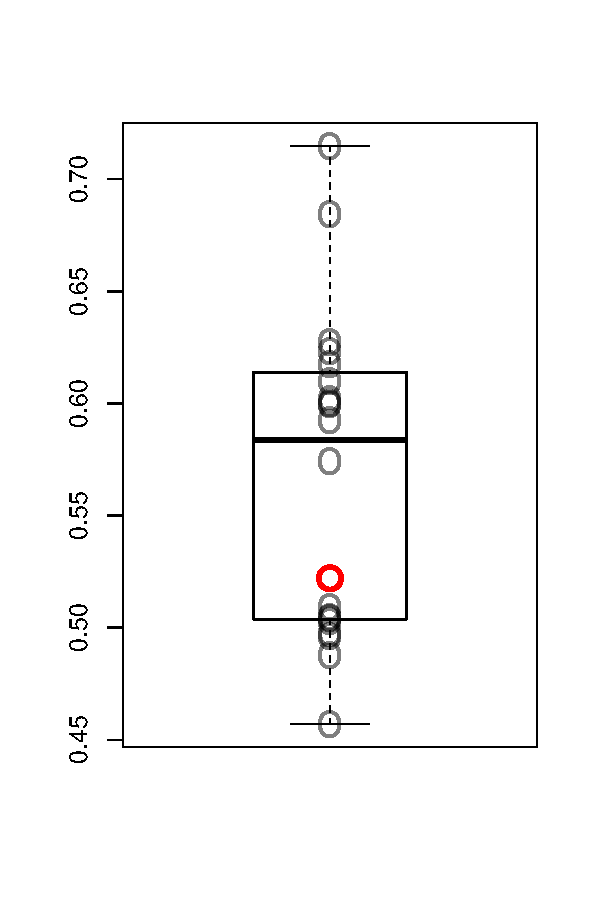
\includegraphics[scale = 0.5]{../extrapolation/autoplots/box4_3.pdf}
\end{column}
\begin{column}{0.5\textwidth}
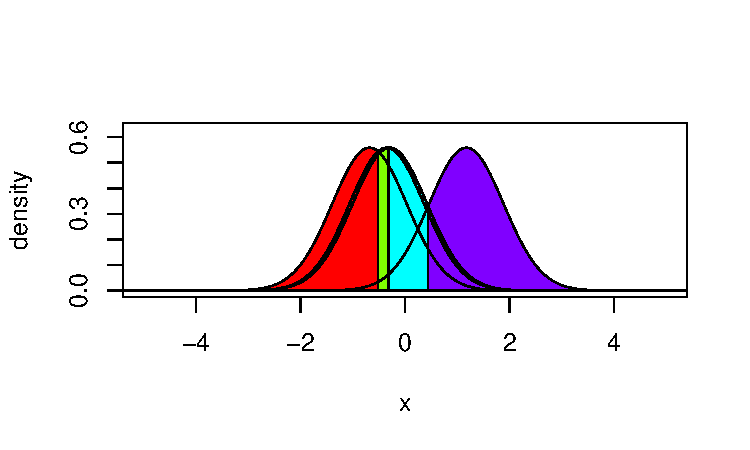
\includegraphics[scale = 0.5]{../extrapolation/autoplots/dens4_3.pdf}
\end{column}
\end{columns}
\end{frame}

\begin{frame}
\frametitle{Toy example}
\begin{center}
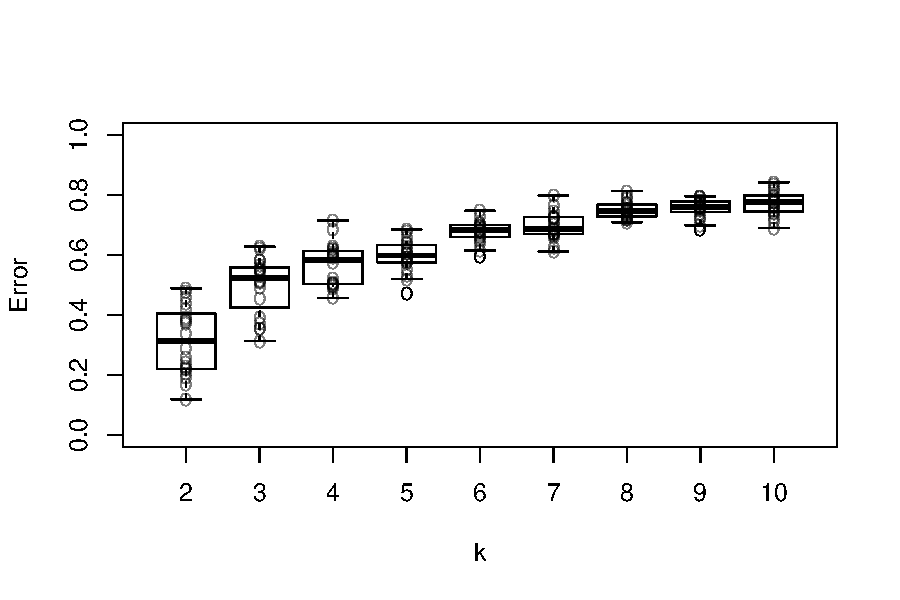
\includegraphics[scale = 0.5]{../extrapolation/autoplots/all_box.pdf}
\end{center}
\end{frame}

\begin{frame}
\frametitle{Toy example}
\begin{center}
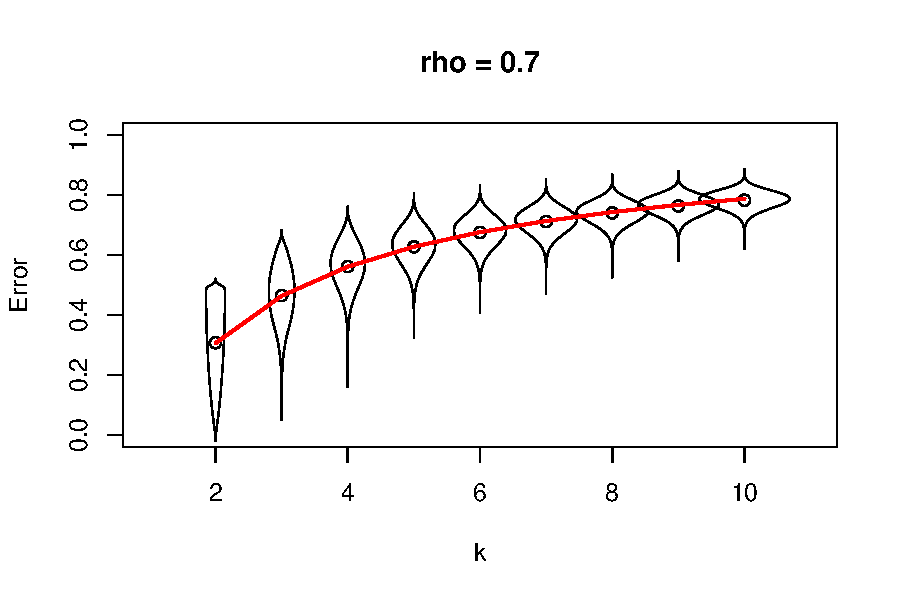
\includegraphics[scale = 0.5]{../extrapolation/illus_err_0_7.pdf}
\end{center}
\end{frame}

\begin{frame}
\frametitle{Computing average risk}
\[
\text{AvRisk}_k = (k-1) \int \bar{D}(u) u^{k-2} du.
\]
\begin{center}
($k$ = 2)
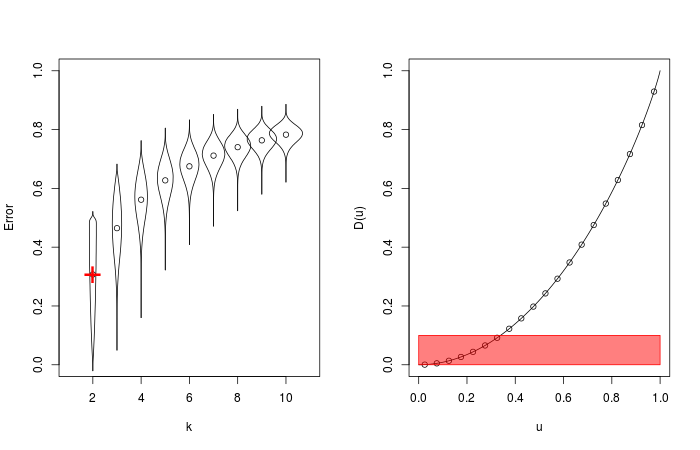
\includegraphics[scale = 0.4, clip=true, trim=0 0.1in 0 0.7in]{../extrapolation/rho_0_7_fmla2.png}
\end{center}
\end{frame}

\begin{frame}
\frametitle{Computing average risk}
\[
\text{AvRisk}_k = (k-1) \int \bar{D}(u) u^{k-2} du.
\]
\begin{center}
($k$ = 3)
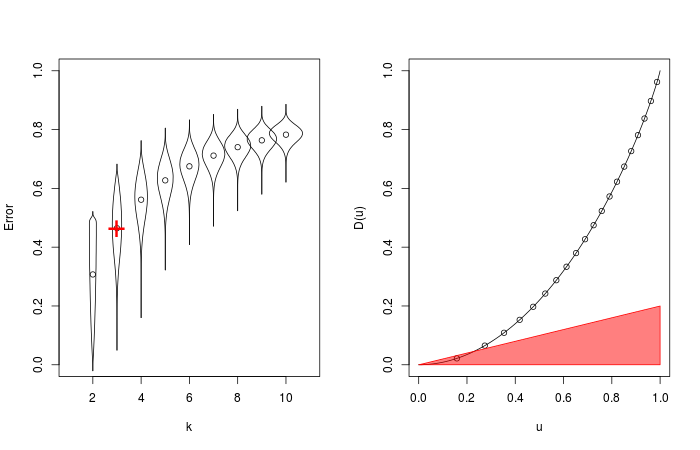
\includegraphics[scale = 0.4, clip=true, trim=0 0.1in 0 0.7in]{../extrapolation/rho_0_7_fmla3.png}
\end{center}
\end{frame}

\begin{frame}
\frametitle{Computing average risk}
\[
\text{AvRisk}_k = (k-1) \int \bar{D}(u) u^{k-2} du.
\]
\begin{center}
($k$ = 4)
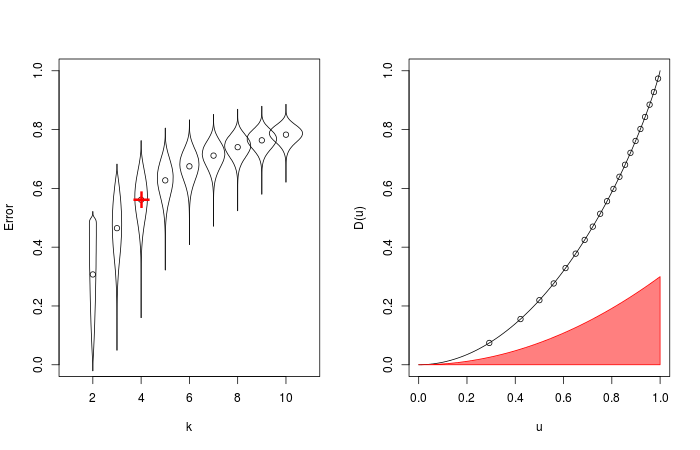
\includegraphics[scale = 0.4, clip=true, trim=0 0.1in 0 0.7in]{../extrapolation/rho_0_7_fmla4.png}
\end{center}
\end{frame}

\begin{frame}
\frametitle{Computing average risk}
\[
\text{AvRisk}_k = (k-1) \int \bar{D}(u) u^{k-2} du.
\]
\begin{center}
($k$ = 5)
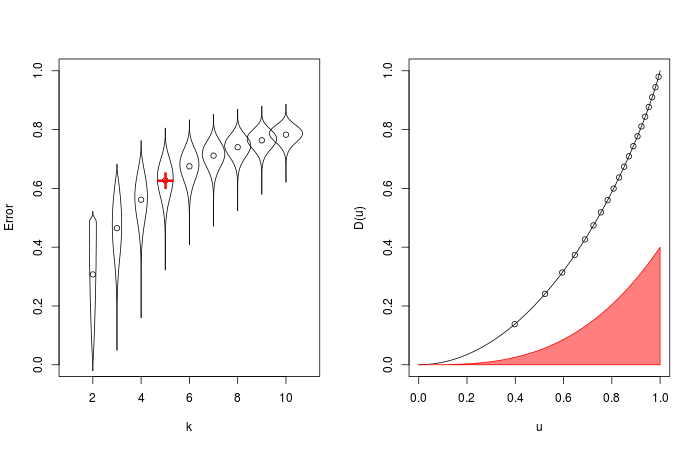
\includegraphics[scale = 0.4, clip=true, trim=0 0.1in 0 0.7in]{../extrapolation/rho_0_7_fmla5.png}
\end{center}
\end{frame}

\begin{frame}
\frametitle{Computing average risk}
\[
\text{AvRisk}_k = (k-1) \int \bar{D}(u) u^{k-2} du.
\]
\begin{center}
($k$ = 6)
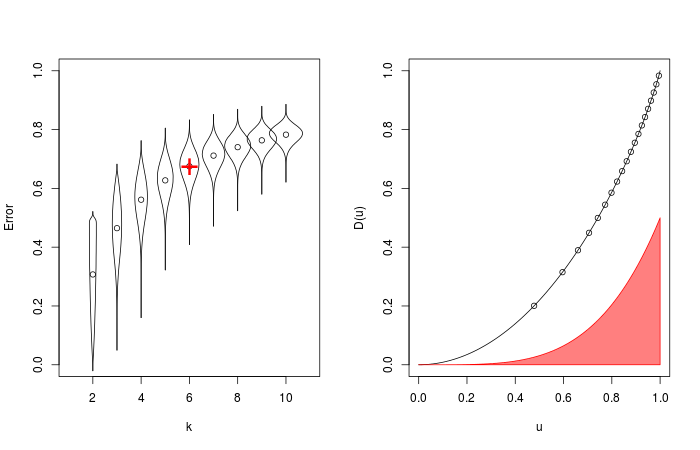
\includegraphics[scale = 0.4, clip=true, trim=0 0.1in 0 0.7in]{../extrapolation/rho_0_7_fmla6.png}
\end{center}
\end{frame}

\begin{frame}
\frametitle{Computing average risk}
\[
\text{AvRisk}_k = (k-1) \int \bar{D}(u) u^{k-2} du.
\]
\begin{center}
($k$ = 7)
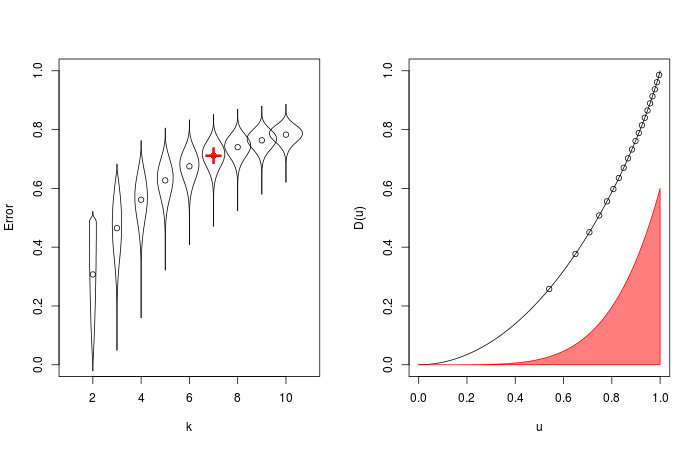
\includegraphics[scale = 0.4, clip=true, trim=0 0.1in 0 0.7in]{../extrapolation/rho_0_7_fmla7.png}
\end{center}
\end{frame}

\begin{frame}
\frametitle{Computing average risk}
\[
\text{AvRisk}_k = (k-1) \int \bar{D}(u) u^{k-2} du.
\]
\begin{center}
($k$ = 8)
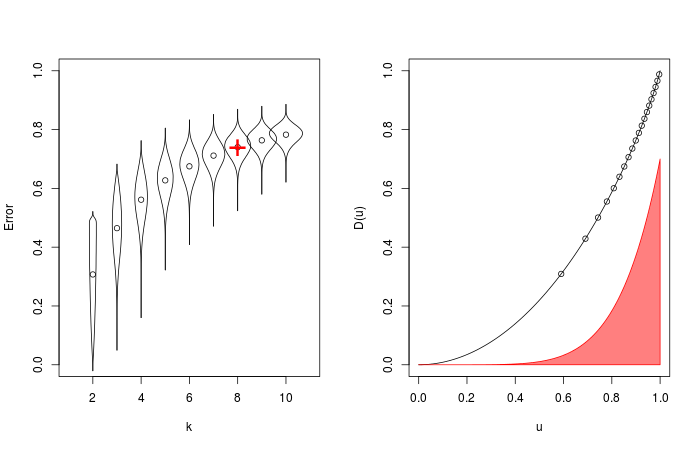
\includegraphics[scale = 0.4, clip=true, trim=0 0.1in 0 0.7in]{../extrapolation/rho_0_7_fmla8.png}
\end{center}
\end{frame}

\begin{frame}
\frametitle{Computing average risk}
\[
\text{AvRisk}_k = (k-1) \int \bar{D}(u) u^{k-2} du.
\]
\begin{center}
($k$ = 9)
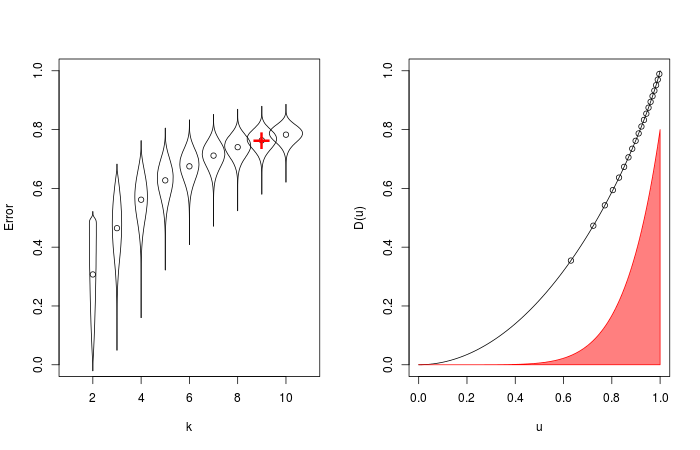
\includegraphics[scale = 0.4, clip=true, trim=0 0.1in 0 0.7in]{../extrapolation/rho_0_7_fmla9.png}
\end{center}
\end{frame}

\begin{frame}
\frametitle{Computing average risk}
\[
\text{AvRisk}_k = (k-1) \int \bar{D}(u) u^{k-2} du.
\]
\begin{center}
($k$ {\tiny =}\hspace{0.025in}10)
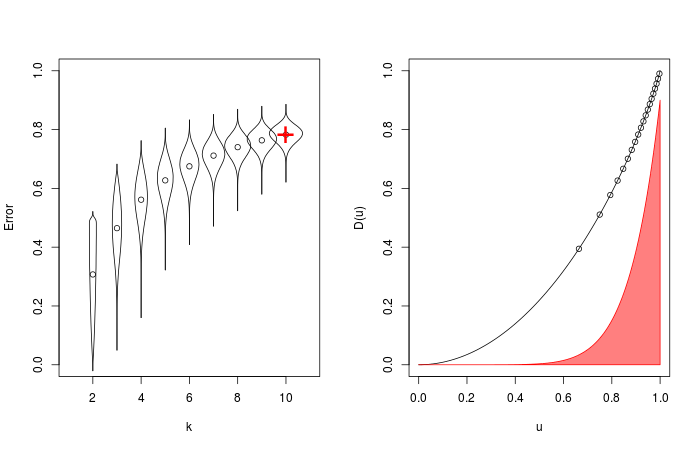
\includegraphics[scale = 0.4, clip=true, trim=0 0.1in 0 0.7in]{../extrapolation/rho_0_7_fmla10.png}
\end{center}
\end{frame}

\begin{frame}
\frametitle{Implication: estimate $\bar{D}(u)$ to predict risk}
\begin{itemize}
\item Theoretical result links $k$-class average risk to $\bar{D}(u)$ function
\item In real data, we do not know $\bar{D}(u)$ since it depends on the unknown joint distribution
\item However, given a model, we can estimate $\bar{D}(u)$
\end{itemize}
\end{frame}

\begin{frame}
\frametitle{Facial recognition example}
\begin{itemize}
\item Data: faces from ``Labeled Faces in the Wild.''
\item 1672 people with at least 2 photos
\item Featurization: trained neural network from OpenFace
\end{itemize}
\begin{center}
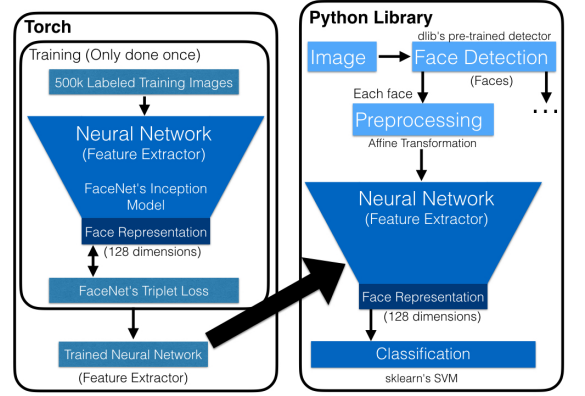
\includegraphics[scale = 0.3]{openface_struc.png}
\end{center}
\end{frame}

\begin{frame}
\frametitle{Facial recognition example}
\begin{columns}
\begin{column}{0.5\textwidth}
\begin{itemize}
\item Let us first subsample 400 faces (out of 1672)
\item Randomly choose 1 face as training and 1 as test for each person
\item Use 1-nearest neighbor.
\begin{itemize}
\item NOTE: 1-NN with 1 example/class is equivalent to LDA with $\Sigma = I$: this fits marginal classifier assumption!
\end{itemize}
\end{itemize}
\pause
\end{column}
\begin{column}{0.5\textwidth}
\begin{center}
\includegraphics[scale = 0.4]{../facerec/acc_plot1.pdf}
\end{center}
\pause
\end{column}
\end{columns}
\vspace{0.1in}
\textbf{Can we predict the accuracy on the full set of 1672?}
\end{frame}

\begin{frame}
\frametitle{Estimated $\bar{D}(u)$}
Using linear spline basis ($p=10000$) and nonnegativity constraint. 
\begin{center}
\includegraphics[scale = 0.5]{../facerec/du_est.pdf}
\end{center}
\end{frame}

\begin{frame}
\frametitle{Estimated risk}
Compare to test risk at $K = 1672$
\begin{center}
\includegraphics[scale = 0.4]{../facerec/acc_plot2.pdf}
\end{center}
\end{frame}

\begin{frame}
\frametitle{Estimated risk: more experiments}
\begin{center}
\begin{tabular}{cc}
\includegraphics[scale = 0.2]{../facerec/sub_100.pdf} &
\includegraphics[scale = 0.2]{../facerec/sub_200.pdf} \\
\includegraphics[scale = 0.2]{../facerec/sub_400.pdf} &
\includegraphics[scale = 0.2]{../facerec/sub_800.pdf}
\end{tabular}
\end{center}
\end{frame}

\begin{frame}
\frametitle{Estimated risk: more experiments}
\begin{center}
\includegraphics[scale = 0.6]{../facerec/sub_preds.pdf}
\end{center}
\end{frame}


\section{Geometry of representations}

\begin{frame}
\sectionpage
\end{frame}



\begin{frame}
\frametitle{Example: face recognition}
\begin{center}
\includegraphics[scale = 0.2]{defense_diagrams/face_2a.png}
\end{center}
In face recognition, the \emph{pose} (including hairstyle) and \emph{lighting} are nuisance parameters.
\end{frame}

\begin{frame}
\frametitle{Example: face recognition}
\begin{center}
\includegraphics[scale = 0.2]{defense_diagrams/face_2b.png}
\end{center}
The same object can map to multiple signals.
\end{frame}

\begin{frame}
\frametitle{What is a representation?}
\begin{center}
\includegraphics[scale = 0.2]{defense_diagrams/representation1.png}
\end{center}
A dimensionality-reducing mapping $\vec{g}$ of the signal.
\end{frame}

\begin{frame}
\frametitle{A good representation...}
\begin{center}
\includegraphics[scale = 0.4]{defense_diagrams/geometry1.png}
\end{center}
\end{frame}

\begin{frame}
\frametitle{A good representation...}
\begin{center}
\includegraphics[scale = 0.4]{defense_diagrams/geometry1a.png}
\end{center}
\end{frame}

\begin{frame}
\frametitle{A good representation...}
\begin{center}
\includegraphics[scale = 0.4]{defense_diagrams/geometry2.png}
\end{center}
\end{frame}

\begin{frame}
\frametitle{...captures the object space geometry}
\begin{center}
\includegraphics[scale = 0.4]{defense_diagrams/geometry2a.png}
\end{center}
\end{frame}

\begin{frame}
\frametitle{Supervised evaluation of representations}
\begin{center}
\includegraphics[scale = 0.25]{defense_diagrams/supervised_eval.png}
\end{center}
\end{frame}

\begin{frame}
\frametitle{Example: face recognition}
\begin{center}
\includegraphics[scale = 0.15]{defense_diagrams/face_3.png}
\end{center}
\begin{itemize}
\item The ID of the individual is an appropriate \emph{response} variable...\pause
\item ...because two photos labeled with the same ID must belong to the same object $\vec{t}$ \pause
\item That is, for $d(y, y')$ being the zero-one distance,
\[
d(y, y') = 0 \Leftrightarrow d(\vec{t}, \vec{t}') = 0.
\]
\end{itemize}

\end{frame}

\begin{frame}
\frametitle{Methods for supervised evaluation of representations}
\begin{itemize}
\item \emph{Triplet loss} (Schroff 2015)
\begin{center}
\includegraphics[scale = 0.3]{../info_theory_paper/thesis_2/Figures/triplet_loss.png}
\end{center}
\pause
\item Average risk of randomized classification (using e.g. 1-nearest neighbor)\pause
\item \emph{Mutual information} $I(g(\vec{Z}), \vec{Y})$
\end{itemize}

\end{frame}


\begin{frame}
\frametitle{Mutual information $I(X; Y)$}
\begin{center}
\includegraphics[scale = 0.23]{shannon_claude.png}
\hspace{0.2in}
\includegraphics[scale = 0.2]{kinney2.png}
\end{center}
Introduced in Shannon's 1948 paper, ``A mathematical theory of communication''
\[
I(X; Y) = \int \log \left(\frac{p(x, y)}{p(x)p(y)}\right) p(x, y) dx dy
\]

\vspace{0.2in}
\tiny{Image credit Kinney et al. 2014.}
\end{frame}

\begin{frame}
\frametitle{Result 1. Lower bound for mutual information}
\begin{itemize}
\item \textbf{Theorem.} (Z., Benjamini 2017) There exists a function $h_k$ such that
\[I(\vec{g}(\vec{Z}); \vec{Y}) \geq h_k(\text{AvRisk}_k).\]
\end{itemize}
\begin{center}
\begin{tabular}{cc}
$h_3$ & $h_4$\\
\includegraphics[scale = 0.4, clip=true, trim=0 0 0 0.55in]{../idloss/g3.pdf} &
\includegraphics[scale = 0.4, clip=true, trim=0 0 0 0.55in]{../idloss/g4.pdf}
\end{tabular}
\end{center}
\end{frame}

\begin{frame}
\frametitle{Result 2. Limiting behavior of accuracy curves} 
(Z., Benjamini 2016)  Define
$\text{ABA}_k$ as the Bayes identification accuracy (or average Bayes
classification accuracy).  Then under a particular high-dimensional
limit,
\begin{equation}\label{abepi}
\text{ABA}_k \approx \pi_k(\sqrt{2 I(X; Y)})
\end{equation}
The function $\pi_k$ is given by
\[
\pi_k(c) = \int_{\mathbb{R}} \phi(z - c)  \Phi(z)^{k-1} dz.
\]
\begin{center}
\includegraphics[scale = 0.2]{piK.png}
\end{center}
\end{frame}

\section*{Acknowledgements}

\begin{frame}
\sectionpage
\end{frame}

\begin{frame}
\frametitle{Co-advisors}
\begin{center}
\includegraphics[scale = 0.04]{IMG_0703.JPG}

\includegraphics[scale = 0.2]{JonathanTreeRot.jpg}
\end{center}
\end{frame}

\begin{frame}
\frametitle{Committee}
\begin{center}
\begin{tabular}{c}
\includegraphics[scale = 0.8]{2014_Efron-indoors.jpg}\\
\includegraphics[scale = 0.19]{poldrack_photo2_400.jpg}\\
\includegraphics[scale = 0.19]{tsachypic.jpg}
\end{tabular}
\end{center}
\end{frame}

\begin{frame}
\frametitle{Collaborators}
\begin{center}
\begin{tabular}{c}
\includegraphics[scale = 0.5]{yuval_b.jpg}\\
\includegraphics[width = 0.3\textwidth]{image3.JPG}
\end{tabular}
\end{center}
\end{frame}

\begin{frame}
\frametitle{{!`}Compadres!}
\begin{center}
\includegraphics[scale = 0.08]{DSCN3957-HDR.jpg}
\end{center}
\end{frame}

\section*{The end}

\begin{frame}
\sectionpage
\end{frame}



\end{document}
\end{frame}
\end{document}


